% Created 2020-07-08 mié 12:49
% Intended LaTeX compiler: pdflatex
\documentclass[presentation,aspectratio=1610]{beamer}
\usepackage[utf8]{inputenc}
\usepackage[T1]{fontenc}
\usepackage{graphicx}
\usepackage{grffile}
\usepackage{longtable}
\usepackage{wrapfig}
\usepackage{rotating}
\usepackage[normalem]{ulem}
\usepackage{amsmath}
\usepackage{textcomp}
\usepackage{amssymb}
\usepackage{capt-of}
\usepackage{hyperref}
\usepackage{khpreamble}
\usepackage{amssymb}
\DeclareMathOperator{\shift}{q}
\DeclareMathOperator{\diff}{p}
\usetheme{default}
\author{Kjartan Halvorsen}
\date{2020-07-08}
\title{Control Computarizado - Discretización de controladores continuosos}
\hypersetup{
 pdfauthor={Kjartan Halvorsen},
 pdftitle={Control Computarizado - Discretización de controladores continuosos},
 pdfkeywords={},
 pdfsubject={},
 pdfcreator={Emacs 26.3 (Org mode 9.3.6)}, 
 pdflang={English}}
\begin{document}

\maketitle


\section{Intro}
\label{sec:orge0e4c3c}
\begin{frame}[label={sec:orgde90e12}]{Retroalimentación Tarea 1}
\begin{itemize}
\item En general \alert{muy buen trabajo} de todos
\item Unos \alert{reportes excelentes}
\item A mejorar: Incluir \alert{referencia a fuente} de cada gráfica
\item Se quedan unos conceptos erróneos
\end{itemize}
\end{frame}

\begin{frame}[label={sec:org551de8e}]{Retroalimentación Tarea 1 - efecto de alias}
 La señal original es un sinusoide de 3Hz \(u(t) = \cos(6\pi t)\),  que tiene la transformada de Fourier 
\[ F(\omega) = \frac{1}{2}\delta(\omega + 6\pi) + \frac{1}{2}\delta(\omega - 6\pi).\]
Se muestrea la señal con  una frecuencia de muestreo de 8Hz, o \(\omega_s = \unit{16\pi}{\rad\per\second}\), que da una frecuencia de Nyquist de \(\omega_N = \frac{1}{2} \omega_s = \unit{8\pi}{\rad\per\second}\). La señal muestreada tiene la transformada de Fourier
  \begin{align*}
   F_s(\omega) &= \frac{1}{h} \sum_{n=-\infty}^\infty F(\omega + n\omega_s) = \frac{1}{h} \left( \cdots + F(\omega - \omega_s) + F(\omega) + F(\omega + \omega_s) + \cdots \right)\\
&= \frac{1}{2h}\Big( \cdots + \big(\delta(\omega -\omega_s + 6\pi) + \delta(\omega -\omega_s - 6\pi)\big)\\& \qquad + \big(\delta(\omega + 6\pi) + \delta(\omega - 6\pi)\big)\\ & \qquad + \big(\delta(\omega +\omega_s + 6\pi) + \delta(\omega +\omega_s - 6\pi)\big) + \cdots \Big)
\end{align*} 
\end{frame}

\begin{frame}[label={sec:orgf727bf5}]{Retroalimentación Tarea 1 - efecto de alias}
\begin{align*}
 F_s(\omega) &= \frac{1}{2h}\Big( \cdots + \delta(\omega -16\pi + 6\pi) + \delta(\omega -16\pi{} - 6\pi)\\& \qquad + \delta(\omega + 6\pi) + \delta(\omega - 6\pi)\\ & \qquad + \delta(\omega +16\pi{} + 6\pi) + \delta(\omega +16\pi{} - 6\pi) + \cdots \Big)
\end{align*} 
\alert{Actividad} Dibuja la transformada de Fourier (espectro) de la señal muestreada!
\begin{center}
  \begin{tikzpicture}[scale=0.3]
  \draw[->] (-23,0) -- (23,0) node[below] {$\omega$};
    \draw[->] (0,-0.2) -- (0,6) node[left] {$|F_s(\omega)|$};
    \foreach \w/\l in {-12/$-12\pi$, -6/$-6\pi$, 0/0, 6/$6\pi$, 12/$12\pi$}
	 \draw (\w, 0) -- (\w, -0.2) node[below] {\l};
  \end{tikzpicture}
\end{center}
\end{frame}
\begin{frame}[label={sec:orgf88c854}]{Transformada de Fourier - solución}
\end{frame}
\begin{frame}[label={sec:orge92865c}]{Transformada de Fourier - solución}
\begin{align*}
 F_s(\omega) &= \frac{1}{2h}\Big( \cdots + \delta(\omega -16\pi + 6\pi) + \delta(\omega -16\pi{} - 6\pi)\\& \qquad + \delta(\omega + 6\pi) + \delta(\omega - 6\pi)\\ & \qquad + \delta(\omega +16\pi{} + 6\pi) + \delta(\omega +16\pi{} - 6\pi) + \cdots \Big)
\end{align*} 

\begin{center}
  \begin{tikzpicture}[scale=0.3]
  \draw[->] (-23,0) -- (23,0) node[below] {};
    \draw[->] (0,-0.2) -- (0,6) node[left] {$|F_s(\omega)|$};
    %\foreach \w/\l in {-12/$-12\pi$, -6/$-6\pi$, 0/0, 6/$6\pi$, 12/$12\pi$}
      %   \draw (\w, 0) -- (\w, -0.2) node[below] {\l};
    \foreach \w/\l in {-22/$-22\pi$, -10/$-10\pi$, -6/$-6\pi$,  6/$6\pi$, 10/$10\pi$, 22/$22\pi$}
	 \draw[red!80!black, ->] (\w, 0) -- (\w, 3) node[pos=0, below] {\l};
    \draw[dashed] (-8, 0) -- (-8,4) node[pos=1, above] {\small $-\omega_N$};
    \draw[dashed] (8, 0) -- (8,4) node[pos=1, above] {\small $\omega_N$};
  \end{tikzpicture}
\end{center}
\end{frame}


\begin{frame}[label={sec:orgbc26f1f}]{Retroalimentación Tarea 1 - Reconstrucción de señales muestreadas}
Reconstrucción de Shannon:
\[ f(t) = \sum_{k=-\infty}^\infty f(kh) \frac{\sin\big(\omega_N(t-kh)\big)}{\omega_N(t-kh)}\]

\begin{itemize}
\item Reconstrucción perfecto de la señal original
\item \alert{No es causal}
\end{itemize}
\end{frame}

\begin{frame}[label={sec:orgfab2401}]{Retroalimentación Tarea 1 - Reconstrucción de señales muestreadas}
Reconstrucción con ROC:
\[ f(t) = f(kh), \quad kh \ge t < kh+h\]
\begin{center}
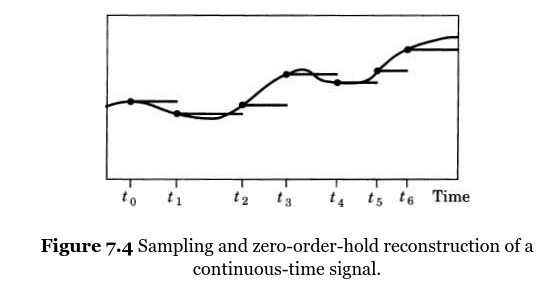
\includegraphics[width=0.6\linewidth]{../../figures/fig7-4.png}\\
{\tiny Åström and Wittenmark \emph{Computer-controlled systems}}
\end{center}

\begin{itemize}
\item \alert{es causal}
\item no es perfecto
\end{itemize}
\end{frame}

\begin{frame}[label={sec:org5349838}]{Retroalimentación Tarea 1 - Reconstrucción de señales muestreadas}
\begin{center}
  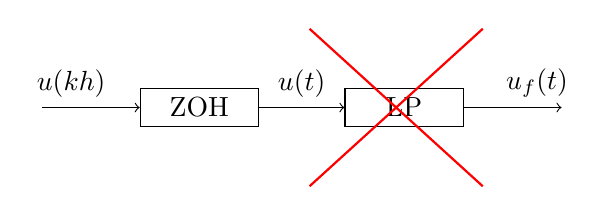
\begin{tikzpicture}[node distance=22mm, block/.style={rectangle, draw, minimum width=15mm}, sumnode/.style={circle, draw, inner sep=3pt}]

    \node[coordinate] (input) {};
    \node[block, right of=input, node distance=20mm] (zoh)  {ZOH};
    \node[block, right of=zoh, node distance=26mm] (lp)  {LP};
    \node[coordinate, right of=lp, node distance=20mm] (output) {};

    \draw[->] (input) -- node[above, pos=0.3] {$u(kh)$} (zoh);
    \draw[->] (zoh) -- node[above] {$u(t)$} (lp);
    \draw[->] (lp) -- node[above, near end] {$u_f(t)$} (output);

    \draw[thick, red] (3.4,-1) to (5.6, 1);
    \draw[thick, red] (3.4,1) to (5.6, -1);
  \end{tikzpicture}
\end{center}
\begin{itemize}
\item Normalmente evitamos un filtro pasobajo en la salida del DAC, porque contribuye un cambio de fase negativo en la gananzia del lazo abierto.
\end{itemize}

\begin{center}
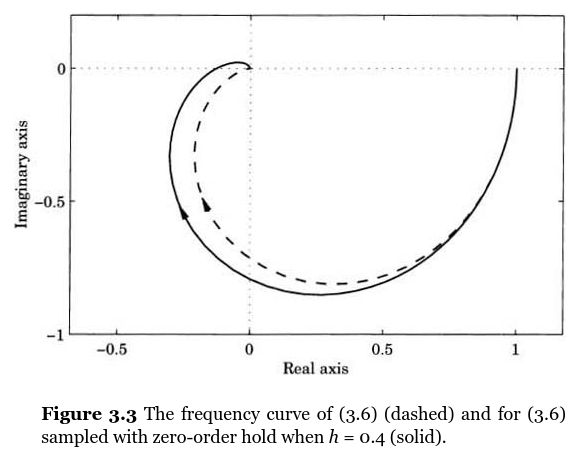
\includegraphics[width=0.4\linewidth]{../../figures/fig3-3.png}
{\tiny Åström and Wittenmark \emph{Computer-controlled systems}}
\end{center}
\end{frame}


\section{Discretization}
\label{sec:org422aac7}
\begin{frame}[label={sec:orgefb03e0}]{Discretización de un controlador continuo}
\end{frame}
\begin{frame}[label={sec:org6a8891a}]{Discretización de un controlador continuo}
\begin{center}
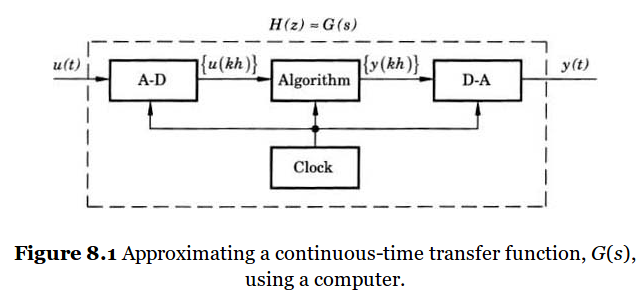
\includegraphics[width=0.7\linewidth]{../../figures/fig8-1.png}
\end{center}

\begin{itemize}
\item Dado un controlador obtenido de un diseño en tiempo continuo
\item Es necesario discretizarlo para implementar en una computadora
\end{itemize}
\end{frame}

\begin{frame}[label={sec:org8ef6db4}]{Position control of a diskdrive arm}
\begin{columns}
\begin{column}{0.5\columnwidth}
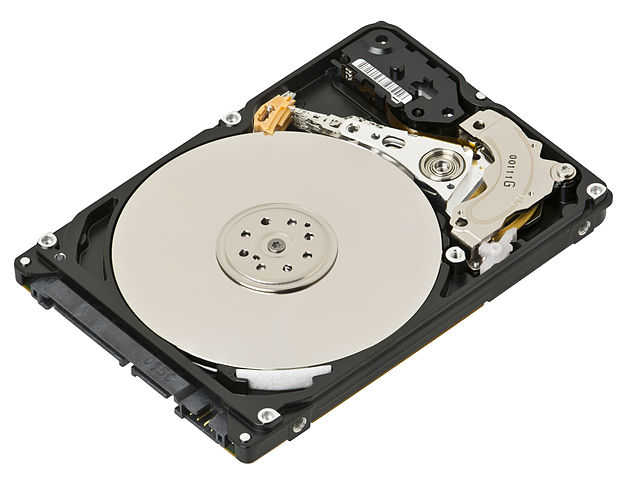
\includegraphics[height=0.5\textheight]{../../figures/diskdrive.png}

\tiny "Laptop-hard-drive-exposed" by Evan-Amos - Own work. Licensed under CC BY-SA 3.0 via Commons
\end{column}
\begin{column}{0.5\columnwidth}
\[ J\ddot{\theta}(t) = u(t) + v(t) \]
\begin{center}
  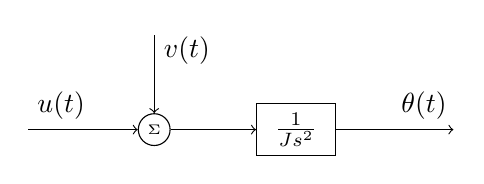
\begin{tikzpicture}[node distance=22mm, block/.style={rectangle, draw, minimum width=10mm}, sumnode/.style={circle, draw, inner sep=2pt}]

    \node[coordinate] (input) {};
    \node[sumnode, right of=input, node distance=16mm] (sum) {\tiny $\Sigma$};
    \node[block, right of=sum, node distance=18mm] (plant)  {$\frac{1}{Js^2}$};
    \node[coordinate, above of=sum, node distance=12mm] (disturbance) {};
    \node[coordinate, right of=plant, node distance=20mm] (output) {};

    \draw[->] (input) -- node[above, pos=0.3] {$u(t)$} (sum);
    \draw[->] (sum) -- node[above] {} (plant);
    \draw[->] (plant) -- node[above, near end] {$\theta(t)$} (output);
    \draw[->] (disturbance) -- node[right, pos=0.2] {$v(t)$} (sum);
  \end{tikzpicture}
\end{center}
\end{column}
\end{columns}
\end{frame}

\begin{frame}[label={sec:orgeafeebf}]{Discretización de un controlador continuo}

\begin{center}
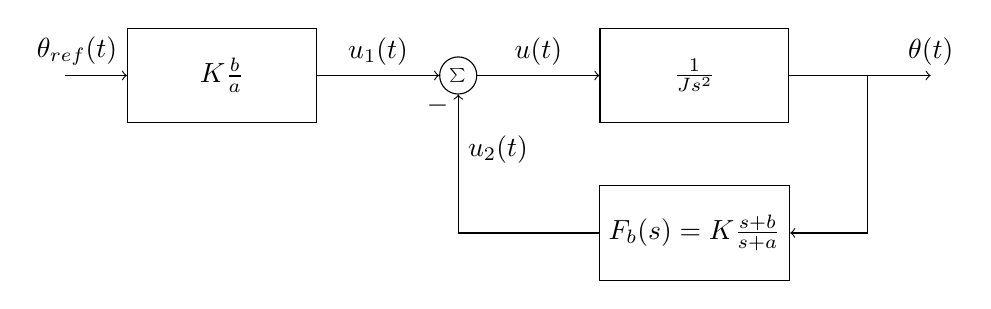
\begin{tikzpicture}
\tikzset{node distance=2cm, 
    block/.style={rectangle, draw, minimum height=12mm, minimum width=24mm},
    sumnode/.style={circle, draw, inner sep=2pt}        
}

  \node[coordinate] (input) {};
  \node[block, right of=input] (TR) {$K\frac{b}{a}$};
  \node[sumnode, right of=TR, node distance=30mm] (sum) {\tiny $\sum$};
  \node[block,right of=sum, node distance=30mm] (plant) {$\frac{1}{Js^2}$};
  %\node[sumnode, right of=plant, node distance=30mm] (sumdist) {$\sum$};
  %\node[coordinate, above of=sumdist, node distance=15mm] (dist) {};
  %\node[coordinate, right of=sumdist, node distance=15mm] (measure) {};
  \node[coordinate, right of=plant, node distance=30mm] (output) {};
  \node[coordinate, right of=plant, node distance=22mm] (measure) {};
  %\node[sumnode,below of=measure, node distance=25mm] (sumnoise) {$\sum$};
  %\node[coordinate, right of=sumnoise, node distance=15mm] (noise) {};
  \node[block,below of=plant, node distance=20mm] (SR) {$F_b(s) = K\frac{s+b}{s+a}$};

  \draw[->] (input) -- node[above, pos=0.2] {$\theta_{ref}(t)$} (TR);
  \draw[->] (TR) -- node[above] {$u_1(t)$} (sum);
  \draw[->] (sum) -- node[above] {$u(t)$} (plant);
  \draw[->] (plant) -- node[at end, above] {$\theta(t)$} (output);
  \draw[->] (measure) |- (SR);
  \draw[->] (SR) -| (sum) node[right, pos=0.8] {$u_2(t)$} node[left, pos=0.96] {$-$};
\end{tikzpicture}
\end{center}
\end{frame}

\begin{frame}[label={sec:org6b53e10}]{Simple discretization}
\begin{center}
\begin{tikzpicture}
\pgfmathsetmacro\tone{2}
\pgfmathsetmacro\ttwo{4}
\pgfmathsetmacro\xone{0.1*\tone*sin(10*\tone)}
\pgfmathsetmacro\xtwo{0.1*\ttwo*sin(10*\ttwo)}
\pgfmathsetmacro\xdot{(\xtwo-\xone)/(\ttwo-\tone)}

\begin{axis}[width=7cm, height=5cm, xtick={\tone, \ttwo}, xticklabels={$t_1$, $t_1+h$},
ytick={\xone, \xtwo}, yticklabels={$x(t_1)$, $x(t_1+h)$}]
\addplot+[no marks, thick, variable=\t, domain = 0:8, samples=100] {0.1*t*sin(10*t)} node[coordinate, pos=0.8, pin=90:{$x(t)$}] {};
\addplot+[ycomb,] coordinates  {(\tone, \xone) (\ttwo, \xtwo)};
\addplot+[this, no marks, variable=\t, domain = -1:3, samples=10] ({\tone + t}, {\xone + \xdot*t});
\end{axis}

\node at (8,3) {\( \dot{x}(t) \approx \frac{\Delta x}{\Delta t} = \frac{x(t + h) - x(t)}{h} \)};
\node at (8,2) {Euler's method}
\end{tikzpicture}
\end{center}

Approximating the controller, assuming equidistant sampling  \(t = kh\):
\begin{align*}
a u_2 + \dot{u}_2 &= Kby + K\dot{y}\\
a u_2(kh) + \frac{1}{h} \big(u_2(kh+h) - u_2(kh)\big) &= Kby(kh) + \frac{K}{h}\big(y(kh+h) - y(kh)\big)
\end{align*}
\end{frame}

\begin{frame}[label={sec:org83c230a}]{Discretización con el método de Euler}
\[ u_2(kh+h) = (1-ah)u_2(kh) + Ky(kh+h) - K(1-bh)y(kh) \]

\alert{Actividad} Es un sistema de primer orden. ¿Cuál es su polo? Marka en el eje real abajo los valores del producto \(ah\) que da un sistema discreto estable.

\begin{center}
  \begin{tikzpicture}
    \draw[->] (-4,0) -- (8,0) node[below] {$ah$};
    \draw (0,-0.1) to (0, 0.1) node[pos=0, below] {0};
    \draw[white] (0,1) to (0,2);
  \end{tikzpicture}
\end{center}
\end{frame}

\begin{frame}[label={sec:org2634602}]{Discretización con el método de Euler - solución}
\end{frame}

\begin{frame}[label={sec:orga8384d6}]{Discretización con el método de Euler - solución}
\[ u_2(kh+h) = (1-ah)u_2(kh) + Ky(kh+h) - K(1-bh)y(kh) \]
\[ u_2(kh) = K \frac{\shift - (1-bh)}{\shift - (1-ah)} y(kh)\]
El polo está en \(1-ah\), y para estabilidad debe tener un magnitúd menos de 1. Es decir 
\[ -1 < (1-ah) < 1\]
\[ -2 < -ah < 0 \]
\[ 0 < ah < 2\]
\begin{center}
  \begin{tikzpicture}
    \draw[->] (-4,0) -- (8,0) node[below] {$ah$};
    \draw (0,-0.1) to (0, 0.1) node[pos=0, below] {0};
    \draw (4,0.1) to (4, -0.1) node[below] {2};
    \draw[white] (0,1) to (0,2);
    \draw[ultra thick, red] (0,0) to (4,0);
  \end{tikzpicture}
\end{center}
\end{frame}


\begin{frame}[label={sec:org0eb00f5}]{Métodos de discretización}
Introduciendo el operador diferencial:  \(\diff f(t) = \frac{d}{dt} f\)

\begin{enumerate}
\item Euler (diferencia hacia adelante) \(\diff \approx \frac{\shift -1}{h}\). Substituir
\[ s = \frac{z-1}{h} \] en \(F(s)\) para obtener
\[ F_d(z) = F(s')|_{s'=\frac{z-1}{h}}. \]
\item Euler hacia atras \(\diff \approx \frac{1 - \shift^{-1}}{h} = \frac{\shift -1}{h\shift}\). Substituir
\[ s = \frac{z-1}{zh} \] en \(F(s)\) para obtener
\[ F_d(z) = F(s')|_{s'=\frac{z-1}{zh}}. \]
\end{enumerate}
\end{frame}

\begin{frame}[label={sec:org3345a0e}]{Métodos de discretización}
\begin{enumerate}
\setcounter{enumi}{2}
\item El método de Tustin (transformada bilineal). Substituir
\[ s = \frac{2}{h}\frac{z-1}{z+1} \] en \(F(s)\) para obtener
\[ F_d(z) = F(s')|_{s'=\frac{2}{h}\cdot \frac{z-1}{z+1}}. \]
\item Discretización invariante a la rampa. Similar a discretización con ROC. La transformada z de una rampa es  \(\frac{zh}{(z-1)^2}\) y su transformada de Laplace \(1/s^2\). La discretización es dado por
\[ F_d(z) = \frac{(z-1)^2}{zh} \ztrf{\laplaceinv{\frac{F(s)}{s^2}}}. \]
\end{enumerate}
\end{frame}

\begin{frame}[label={sec:org57598b5}]{Deformación del eje de frecuencias con el método de Tustin}
\begin{center}
 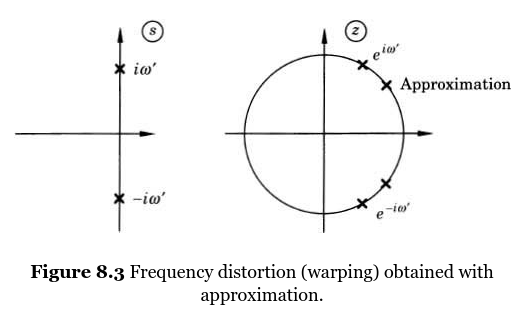
\includegraphics[width=0.6\linewidth]{../../figures/fig8_3.png}\\
{\tiny Åström and Wittenmark \emph{Computer-controlled systems}}
\end{center}
El eje imaginario del plano \(s\), infintamente largo, se mapea al circulo unitario del plano \(z\), que es finito.
\end{frame}
\begin{frame}[label={sec:orge22b8d3}]{Mapeo de la región estable del plano \(s\)}
\begin{center}
 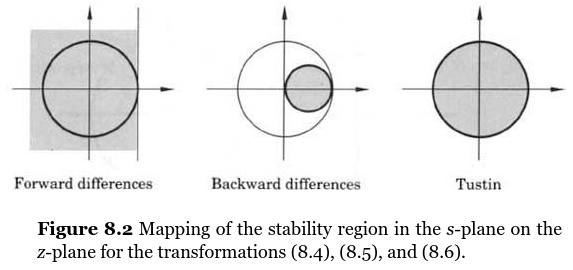
\includegraphics[width=0.79\linewidth]{../../figures/fig8-2.png}\\
{\tiny Åström and Wittenmark \emph{Computer-controlled systems}}
\end{center}
\end{frame}

\begin{frame}[label={sec:org87ef9f3}]{Ejercicio}
\alert{En pares} Divida entre ustedes los dos ejercicios abajo. Despues de 5 minutos explica su procedimiento y resultado a su compañer@.

Determine la approximación del compensador lead \(F(s) = \frac{s+b}{s+a}\), y el polo de la approximación.
\begin{enumerate}
\item Euler hacia atras
\[ F_d(z) = F(s')|_{s'=\frac{z-1}{zh}}. \]
\item Tustin
\[ F_d(z) = F(s')|_{s'=\frac{2}{h}\cdot \frac{z-1}{z+1}}. \]
\end{enumerate}
\end{frame}
\begin{frame}[label={sec:orge0775c3}]{Forward difference exercise}
\begin{center}
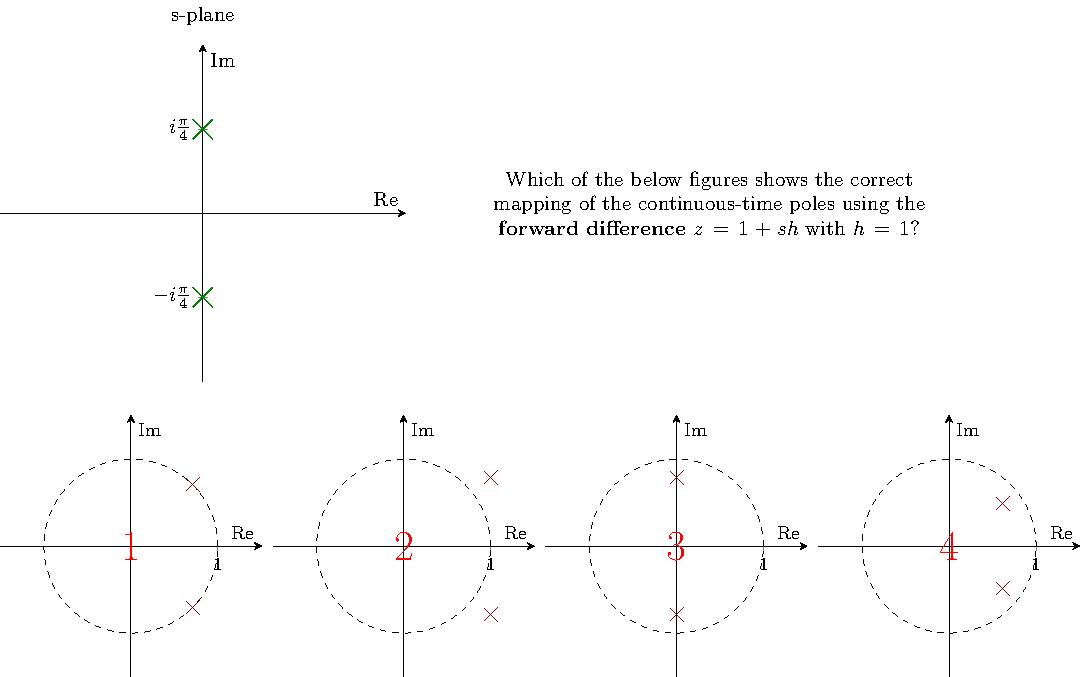
\includegraphics[width=\linewidth]{../../figures/forward-diff-exercise}
\end{center}
\end{frame}

\begin{frame}[label={sec:orgc9ecb93}]{Backward difference exercise}
\begin{center}
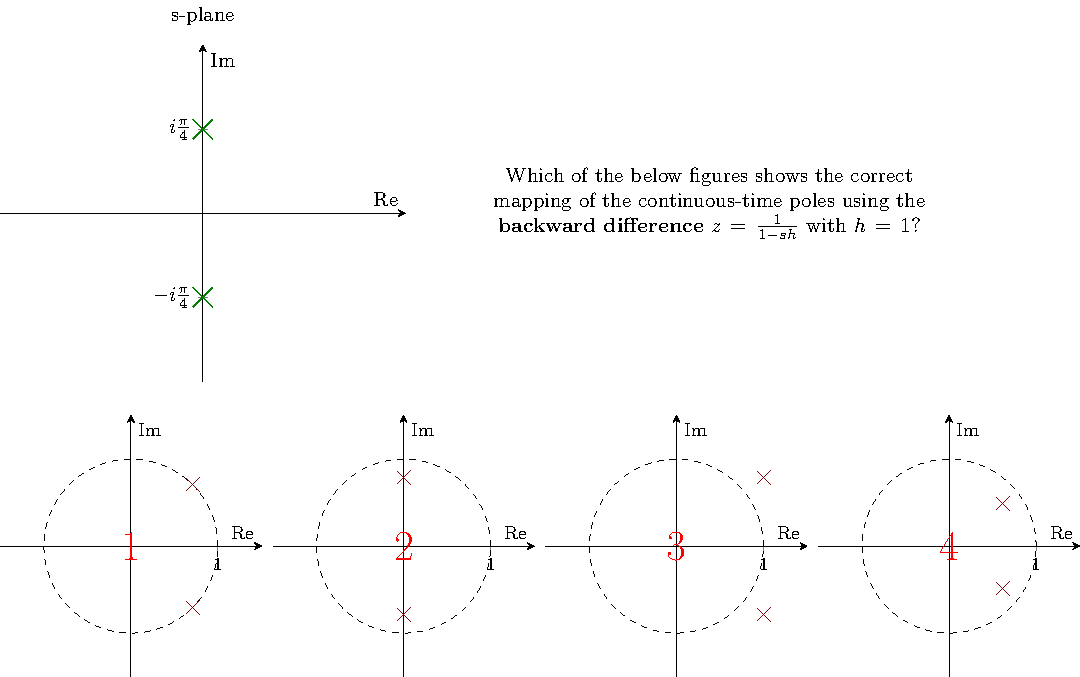
\includegraphics[width=\linewidth]{../../figures/backward-diff-exercise}
\end{center}
\end{frame}
\end{document}